\documentclass{article}
\usepackage[utf8]{inputenc}
\usepackage{indentfirst}
\usepackage{titling}
\usepackage{geometry}
\usepackage{graphicx}
\graphicspath{ {./Images/} }
\usepackage[shortlabels]{enumitem}
\usepackage{fancyhdr}
\usepackage{ulem}
\usepackage[dvipsnames]{xcolor}
\usepackage{amssymb}
\usepackage{listings}
\usepackage{color}

\definecolor{dkgreen}{rgb}{0,0.6,0}
\definecolor{gray}{rgb}{0.5,0.5,0.5}
\definecolor{mauve}{rgb}{0.58,0,0.82}

\lstset{frame=tb,
  language=Java,
  aboveskip=3mm,
  belowskip=3mm,
  showstringspaces=false,
  columns=flexible,
  basicstyle={\small\ttfamily},
  numbers=none,
  numberstyle=\tiny\color{gray},
  keywordstyle=\color{blue},
  commentstyle=\color{dkgreen},
  stringstyle=\color{mauve},
  breaklines=true,
  breakatwhitespace=true,
  tabsize=3
}

\def\ojoin{\setbox0=\hbox{$\bowtie$}%
  \rule[-.02ex]{.25em}{.4pt}\llap{\rule[\ht0]{.25em}{.4pt}}}
\def\leftouterjoin{\mathbin{\ojoin\mkern-5.8mu\bowtie}}
\def\rightouterjoin{\mathbin{\bowtie\mkern-5.8mu\ojoin}}
\def\fullouterjoin{\mathbin{\ojoin\mkern-5.8mu\bowtie\mkern-5.8mu\ojoin}}

\renewcommand\maketitlehooka{\null\mbox{}\vfill} %para centralizar verticalmente
\renewcommand\maketitlehookd{\vfill\null}
\pagestyle{fancy}
\fancyhf{}
\rfoot{\thepage}
\lfoot{ 
\includegraphics[scale=0.01]{UA.jpg} José Mendes 107188 LEI}
\geometry{
  a4paper,
  headheight=4cm,
  top=5.5cm,
  bottom=4.5cm,
  footskip=4cm
}


\title{Tecnologias e Programação Web - Teste 2}
\author{José Mendes 107188}
\date{2023/2024}

\begin{document}


\begin{titlepage}
    \maketitle
    \begin{center}
        
\includegraphics[scale=0.4]{UA.png}
    \end{center}
    \thispagestyle{empty} %remove o count da pagina
\end{titlepage}

\pagebreak

\section{Angular Framework}

\subsection{Typescript}

Começa da mesma sintaxe e semântica que o JavaScript. Consegue usar código JavaScript
existente, incorporar bibliotecas JavaScript bastante populares e o seu código
compilado pode ser chamado a partir de JavaScript.

\vspace{2mm}

Typescript compila para código JavaScript simples, legível e \textbf{compatível com qualquer
navegador, Node.js e qualquer engine que suporte ECMAScript 3} (ou superior).

\vspace{2mm}

A melhor parte do Typescript é o uso de \textbf{Types} em JavaScript.
Mesmo sendo opcional. Desta forma permite práticas JavaScript como:
\begin{itemize}
  \item \textbf{Static Checking} - deteção de erros em tempo de compilação
  \item \textbf{Code Refactoring} - alterar o código sem alterar o comportamento
\end{itemize}

Os tipos deixam definir interfaces entre componentes de software, dando mais
controlo no comportamento de bibliotecas JavaScript.
O Typescript também permite \textbf{type inference} para verificação
estática de código.

\subsubsection{Declaração de Variáveis}

\begin{lstlisting}
  var x = 1; // deprecated because its flaws

  let y = 2; // new and strong declaration

  const z = 3; // constants

  let arr = [10, 20];
  let [a, b] = arr; // array destructuring

  Let o = { a: 1, b: 'hello', c: 10 }
  Let {a, c} = o; // object destructuring
\end{lstlisting}

\pagebreak

\subsubsection{Tipos Básicos}

\begin{lstlisting}
  // boolean
  let isfull: boolean = true;

  // number
  let dec: number = 10.5; // decimal
  let hex: number = 0xFF; // hexadecimal
  let oct: number = 0o373 // octal
  let bin: number = 0b1010 // binary

  // string
  let name: string = "John";
  name = 'Jones';
  let s: string = 'Your name is: ${name}';

  // array
  let list: number[] = [10, 20, 30];
  let list: Array<number> = [10, 20, 30];

  // tuple
  let t: [Boolean, number];
  t = [false, 100]; // ok
  t = [100, false]; // error

  // enum
  enum Color {red, green, blue}
  let c: Color = Color.green;

  // any
  let what: any = 100;
  what = true; // ok

  // void (nothing, the opposite of any)
  let nothing: void = null; // or undefined, normally used for return type of a function

  // null and undefined
  // null is the absence of a value in a variable
  // undefined is the absence of definition of a variable

  // never
  // type of values that never occur
  // usually used as function type for never ending functions

  // type assertions (cast like)
  let avalue: any = "this is a string value";
  let slength: number = (<string>avalue).length;
\end{lstlisting}

\pagebreak

\subsubsection{Funções}

Tal como em JavaScript, as funções podem ser criadas tanto como
com nome ou anónimas, e tipadas.

\begin{lstlisting}
  function add(x: number, y: number): number {
    return x + y;
    }
  let sum = add(1, 2);
  // or:
  let sum = function(x: number, y: number): number {
    return x + y;
  };
\end{lstlisting}

Definir o tipo das funções:
\begin{itemize}
  \item Inclui 2 partes, parametros e tipo de retorno
  \item Na função seguinte, tem de ter 2 parametros do tipo number e retorna um number
\end{itemize}

\begin{lstlisting}
  let sum: (a: number, b: number) => number =
    function(x: number, y: number): number {
      return x + y;
    };
\end{lstlisting}

Pode ter parametros \textbf{default}:

\begin{lstlisting}
  function myname(fname: string, lname: 'Burton') {
    return fname + " " + lname;
  }
\end{lstlisting}

Parametros \textbf{opcionais}:

\begin{lstlisting}
  function myname(fname: string, lname?: string) {
    if (lname)
      return fname + " " + lname;
    else
      return fname;
  }
\end{lstlisting}

Funções \textbf{Fat Arrow}:

\begin{lstlisting}
  let sum = (a, b) => a + b;
  s = sum(10, 20);
  
  // or

  let data = [1, 2, 3];
  let s = 0;
  data.forEach((x) => s += x);
\end{lstlisting}

\pagebreak

\subsubsection{Interfaces}

Um dos principios base do Typescript é que a verificação de tipo se concentra
na forma que os valores têm.

São uma forma poderosa de definir contratos dentro do código, bem como contratos
com código exterior.

\begin{lstlisting}
  interface Hello {
    mesg: string;
    name: string;
  }

  function printHello(obj: Hello)
  {
    console.log(obj.mesg + " " + obj.name + "!!!");
  }

  let myObj = {idobj: 10, mesg: "Hello myfriend", name: "John",
              fullname: "John Simons"};
  printHello(myObj); // Hello myfriend John!!!
\end{lstlisting}

\subsubsection{Classes}

O Typescript permite aos desenvolvedores usar técnicas de programação orientada
a objetos, baseada em classes, para programar os seus web scripts.

Compila para código JavaScript que funciona em qualquer browser moderno
e plataformas, sem ter de esperar pela próxima versão do JavaScript.

\begin{lstlisting}
  class Welcome {
    name: string;
    constructor(name: string) {
      this.name = name;
    }
    say() {
      return 'Hello ${this.name}! You`re Welcome!!!';
    }
  }

  let w = new Welcome("Robert");
  console.log(w.say());
\end{lstlisting}

\pagebreak

\subsubsection{Classes - Herança}

\begin{lstlisting}
  class Person {
    name: string;
    constructor(name: string) {
      this.name = name;
    }
    say() {
      return 'Hello ${this.name}!';
    }
  }

  class Employee extends Person {
    id: number;
    constructor(name: string, id: number) {
      super(name);
      this.id = id;
    }
    say() {
      return super.say() + ' Your id is: ${this.id}';
    }
  }

  let e = new Employee("Robert", 100);
  console.log(e.say());
\end{lstlisting}

\subsubsection{Classes - Overloading}

\begin{lstlisting}
  class Animal {
    name: string;
    constructor(n: string){
      this.name = n;
    }
    talk() {
      return this.name + " is talking: ";
    }
  }
  class Dog extends Animal {
    constructor(name: string){
      super(name);
    }
    talk() {
      return super.talk() + 'Woof! Woof!';
    }
  }
  let dog = new Dog('Ben');
  let ss = dog.talk();
  console.dog(ss);
\end{lstlisting}

\pagebreak

\subsubsection{Modules}

\begin{itemize}
\item \textbf{Modules} são executados dentro de seu próprio escopo, não no escopo global;
\item Variáveis, dunções, classes, etc, declaradas em um módulo não são visíveis fora do módulo;
\item \textbf{Modules} são declarativos - relações entre módulos são especificadas
em termos de \textbf{imports} e \textbf{exports} ao nível do ficheiro;
\item Em Typescript, qualquer ficheiro contendo um top-level \textbf{import} ou
\textbf{export} é considerado um módulo.
\item Qualquer ficheiro sem um top-level \textbf{import} ou \textbf{export}
é tratado como um script com conteúdos disponíveis no escopo global.
\end{itemize}

\begin{lstlisting}
  // File: Validation.ts
  export interface StringValidator {
    isAcceptable(s: string): boolean;
  }
  // File: ZipCodeValidator.ts
  import { StringValidator } from "./Validation";
  export const numberRegexp = /^[0-9]+$/;
  export class ZipCodeValidator implements StringValidator {
    isAcceptable(s: string) {
      return s.length === 5 && numberRegexp.test(s);
    }
  }
\end{lstlisting}

\subsection{Angular}

A \textbf{Angular Framework} é uma aplicação de desenvolvimento web baseada em
linuagem \textbf{TypeScript}.

Faz a transição de MVC (Model-View-Controller), usado em AngularJS, para uma abordagem
\textbf{Components-Based Web Development}.

O \textbf{Angular} permite construir aplicações web através de componentes,
que são blocos de construção UI, fáceis de testar e reutilizar.

Estes componentes encapsulam bem todo o estilo e a função necessária para uma
determinada feature, criando elementos HTML personalizados.

\vspace{2mm}

A ideia é construir componentes declarativos, completmente encapsulados. Estes descrevem as
próprias views, e podem ser facilmente packaged e distribuidos para outros developers.

A aplicação consiste de um componente \textbf{root} que contém um conjunto de
componentes para cada elemento UI, screen e route.

Esta árvore de componentes é a base de qualquer aplicação Angular.

\pagebreak

\subsection{Angular - Arquitetura}

\begin{center}
  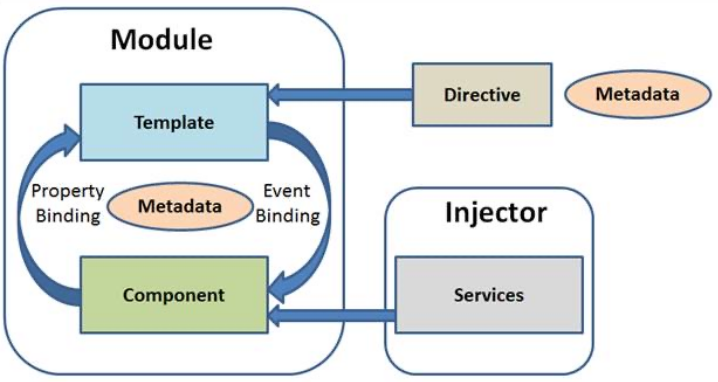
\includegraphics[scale=0.4]{1}
\end{center}

\subsubsection{Modules}

\begin{itemize}
\item É um bloco de códifo com o objetivo de realizar uma única tarefa simples.
\item Pode ser exportado em forma de classe.
\item Aplicações Angular podem ter vários modules, no entanto, têm de ter pelo menos 1.
\item Cada aplicação Angular tem um \textbf{root module}, que pode ter vários
\textbf{feature modules}.
\end{itemize}

Um módulo Angular é uma classe com o decorador \textbf{@NgModule}. Decoradores,
fornecem uma forma de adicionar anotações e sintaxe meta-programática
para declaração de classes e membros.

\textbf{@NgModule} pega num único objeto de metadados e as suas propriedades
para descrever o módulo.

\begin{center}
  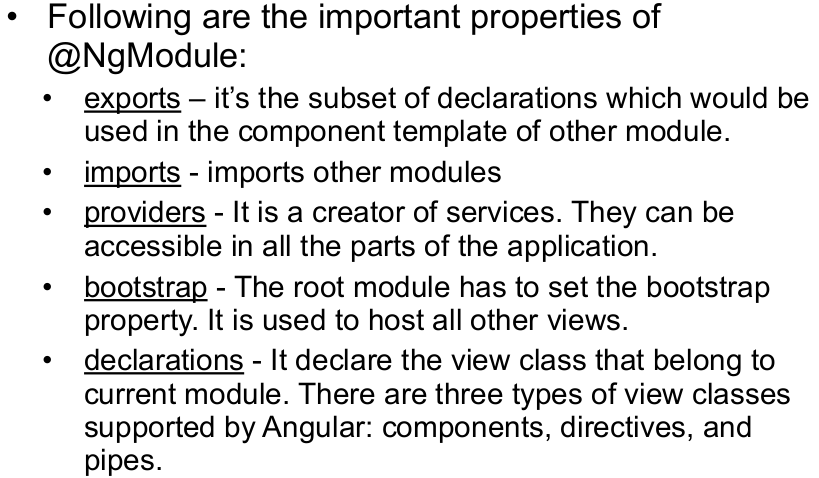
\includegraphics[scale=0.3]{2}
\end{center}

\pagebreak

\subsection{Angular - Components}

Um componente é uma combinação de uma classe, que contém a lógica base para uma página,
e um template associado que trata da view.

A lógica da aplicação é escrita dentro da classe que é usada pela view.
A classe interage com a View através de métodos e propriedades da sua API.

O Angular cria e dá update dos componentes conforme necessário, e destrói os
que já não são usados, enquanto o utilizador navega pela aplicação.

\subsection{Angular - Metadados}

Os metadados é a forma como o Angular processa uma classe, um método ou uma propriedade.
Em Typescript, os metadados são representados por decoradores.
Por exemplo, o decorador \textbf{@Component} é usado para definir um componente.

\subsection{Angular - Template}

Um template é a view de um componente e diz ao Angular como renderizar o componente.
É semelhante ao HTML normal.

\subsection{Angular - Data Binding}

O \textbf{Data Binding} é uma feature poderosa do desenvolvimento de software.
É a conexão entre a View e a lógica de negócio da aplicação.

\vspace{2mm}

Há 4 tipos de \textbf{Data Binding} suportados pelo Angular:

\begin{center}
  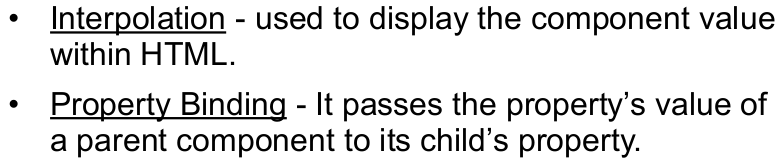
\includegraphics[scale=0.3]{3}
  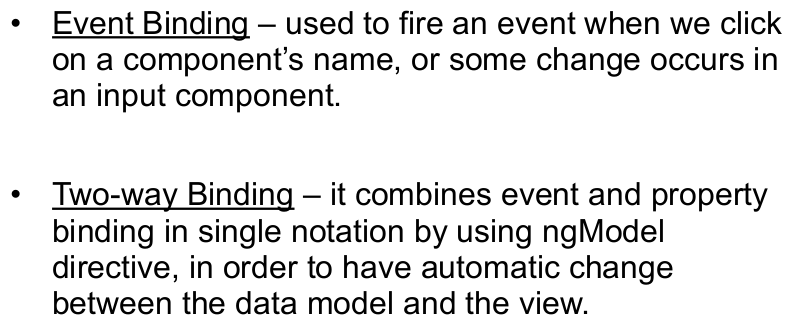
\includegraphics[scale=0.3]{4}
\end{center}

\pagebreak

\subsection{Angular - Diretivas}

As diretivas extendem o HTML com atributos. Estes marcadores nos elementos
do DOM têm um comportamento especial e dizem ao Angular HTML compiler para
anexar.

\begin{center}
  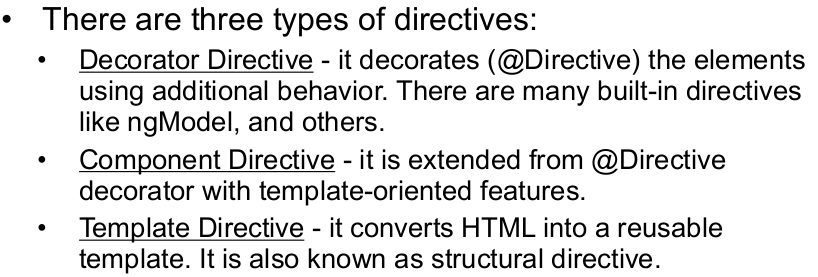
\includegraphics[scale=0.3]{5}
\end{center}

\subsection{Angular - Service}

\begin{itemize}
  \item Um \textbf{Service} é uma categoria vasta que engloba qualquer valor,
  função ou feature que a aplicação necessite.
  \item Um serviço é tipicamente uma classe com um propósito bem definido.
  \item O Angular distingue componentes de serviços para aumentar a modularidade e a reusabilidade.
  \item Tipicos exemplos de serviços são: logging service, data service, message bus, etc.
\end{itemize}

\subsection{Angular - Dependency Injection}

\begin{itemize}
  \item O \textbf{Dependency Injection} é um padrão de design de software
  em quais os objetos são passados como dependências.
  \item Ajuda-nos a remover as dependências hard-coded e torna as dependências configuráveis.
  \item Usar \textbf{Dependency Injection} pode tornar componentes mais maintainable, reusable, and
  testable.
  \item DI está conectado à Angular Framework e usado em toda a aplicação,
  para fornecer novos componentes com os serviços ou outras coisas que necessitam.
\end{itemize}

\pagebreak

\subsection{Angular - Routing}

O browser é um modelo familiar para navegação de uma aplicação.
Introduzir um URL na barra de endereço para ir para uma página, clicar em links
para ir para uma página nova, usar os butões de voltar e de avançar para navegar.

\vspace{2mm}

O \textbf{Angular Router} é baseado nesse modelo:
\begin{itemize}
  \item Consegue interpretar um URL como uma instrução para navegar para uma client-generated view.
  \item Podem se passar parametros opcionais, ajudando a view a mostrar os detalhes da informação.
  \item Podemos estabelecer links numa página para ajudar o utilizador a navegar, clicando nos links.
  \item Podemos navegar imperativamente quando o utilizador clica num botão ou seleciona de uma lista.
  \item E os logs de navegação mantêm o histórico do browser, permitindo usar os botões de voltar e de avançar.
\end{itemize}

\subsubsection{Desenvolvimento}

A melhor forma é dando load e configurando o router de forma separada e top-level module
que é dedicado ao routing.
Por convenção, este módulo fica em \textbf{"app.routes.ts"} no
diretório \textbf{"src/app"}, que exporta \textbf{Routes}.

\subsubsection{Adicionando Routes}

\begin{center}
  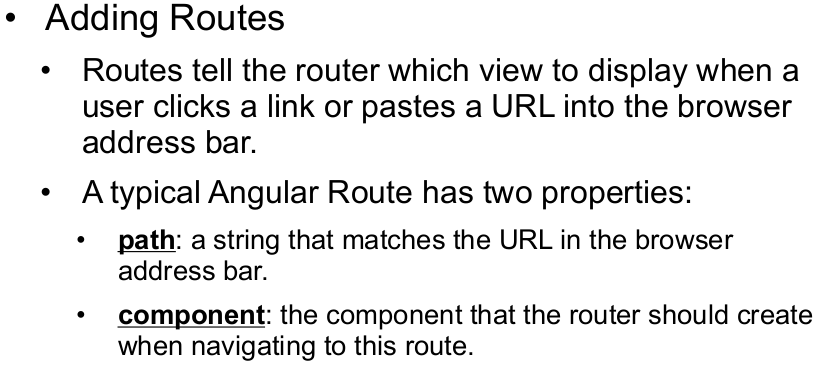
\includegraphics[scale=0.3]{6}
  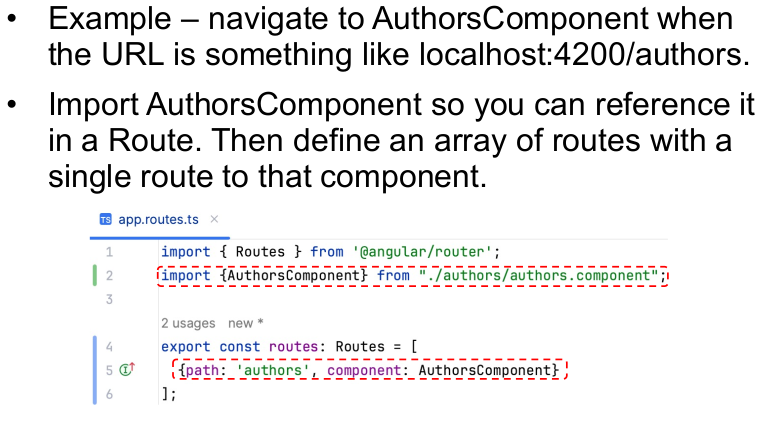
\includegraphics[scale=0.3]{7}
  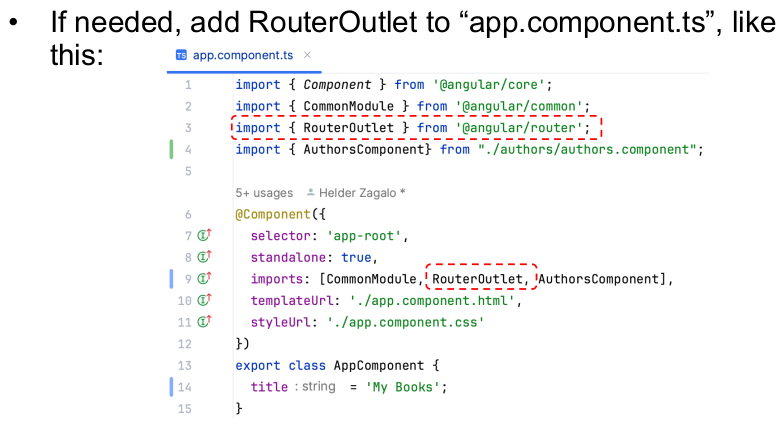
\includegraphics[scale=0.3]{8}
  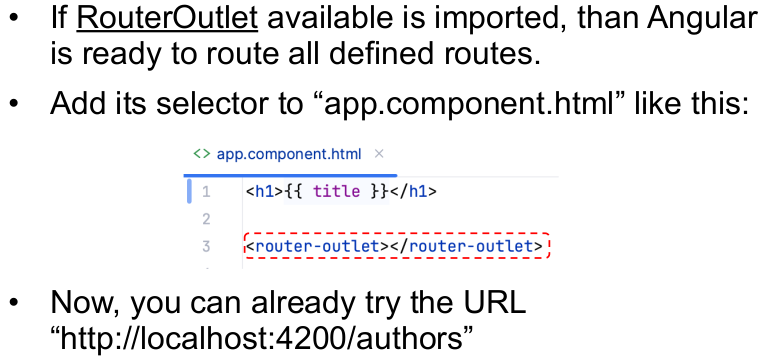
\includegraphics[scale=0.3]{9}
  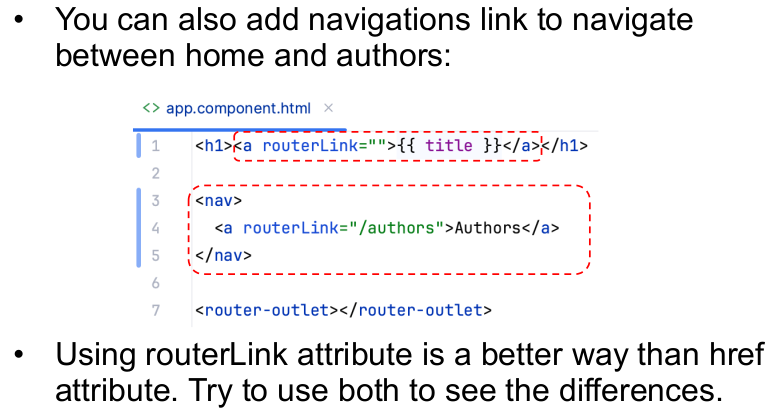
\includegraphics[scale=0.3]{10}
\end{center}

\section{Django Framework}

\subsection{RESTful Web Services - Django REST Framework}

\subsubsection{Serviços Web}

Os serviços web são serviços oferecidos por dispositivos eletrónicos
para enviar dados para outros dispositivos eletrónicos, usando tecnologias web.

Normalmente, os dados são enviados em formato XML ou JSON.

Um de muitos propósitos de serviços web é para fornecer interoperabilidade e
integração dos dados entre sistemas de informação heterogéneos.

\subsubsection{REST Web Services}

\textbf{REST} significa \textbf{REpresentational State Transfer}.

É um modelo de arquitetura para aplicações hypermedia, maioritariamente usado para
implementação de serviços web, sendo leve, simples, escalável e sustentável.

Um serviço baseado nesta tecnologia designa-se por \textbf{RESTful Service}.

Serviços REST, não dependem de nenhum protocolo específico, mas o mais usado é
o \textbf{HTTP} para transportar os dados.

Outro tipo de serviços web, são os \textbf{SOAP Web Services}, que são baseados
no protocolo \textbf{SOAP}, que é muito formal, restrito e pesado, pelo que não são
tão populares como os RESTful.

\subsubsection{Django REST Framework (DRF)}

O DRF é uma biblioteca python para criar serviços web RESTful integrados
na Framework Django.

Fornece um conjunto de funções importantes para programar os seguintes serviços:
\begin{itemize}
  \item A possibilidade de publicar uma dada API.
  \item Politicas de autenticação, usando \textbf{OAuth1} ou \textbf{OAuth2}.
  \item Serialização de dados de BDs através do ORM do Django.
  \item Pode usar views genéricas, caso não seja necessário personalizar as views.
  \item Atualmente é usado em grandes organizações como \textbf{Mozilla}, \textbf{Red Hat}, \dots
\end{itemize}

\end{document}